\begin{figure*}[t]
  \centering
  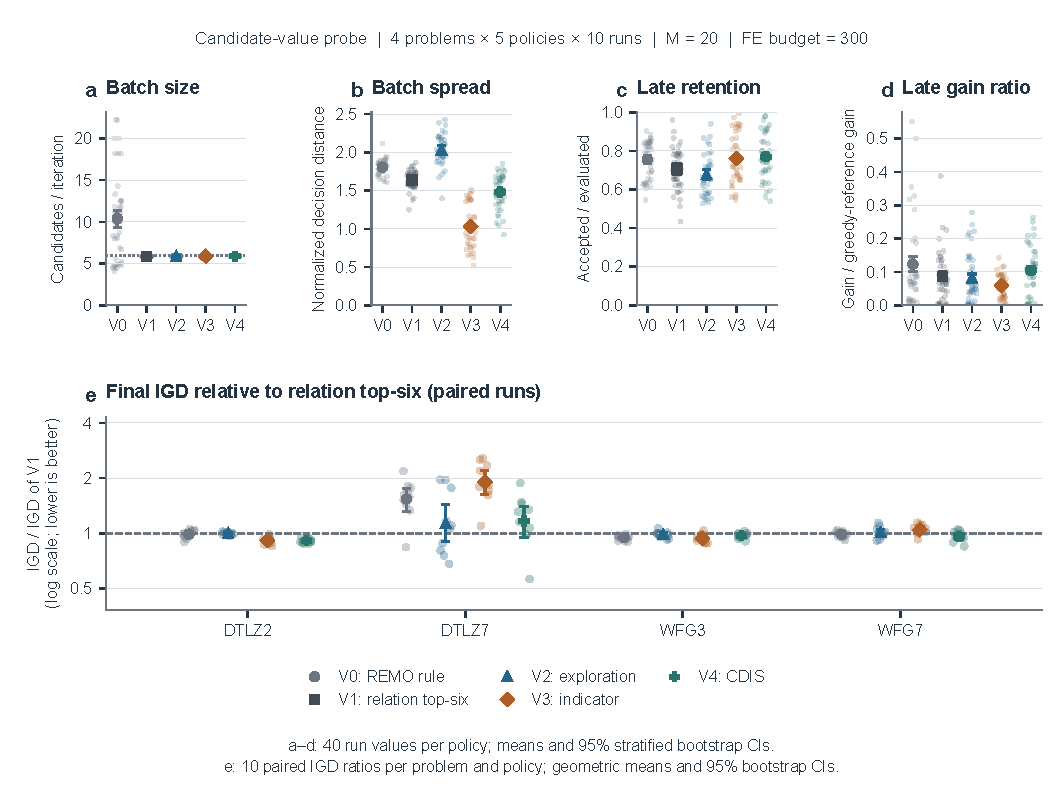
\includegraphics[width=0.98\textwidth]{figures/fig_candidate_evidence.pdf}
  \caption{Candidate-value probe on four 20-objective problems at
  $FE_{\max}=300$. (a--d)~Batch size, decision-space spread, late-stage
  retention and within-pool gain ratio. Faint dots are all 40 run-level values
  per policy; larger markers show equally weighted means over problems and
  runs, with 95\% percentile bootstrap confidence intervals from 4,000
  within-problem run resamples. Batch size and spread use the full trajectory;
  retention and gain ratio use $FE/FE_{\max}\geq0.5$.
  (e)~Final IGD divided by that of V1 on the same problem and seed. Each group
  contains ten paired ratios; markers and intervals are geometric means and
  95\% bootstrap confidence intervals, calculated on log ratios. Values below
  one favor the displayed policy. V0 applies the REMO rule in the probe host;
  V1--V4 respectively use relation top-six, exploration, indicator and
  CDIS. Each closed-loop run generates its own candidate pools.
  \label{fig:candidate-evidence}}
\end{figure*}
